\begin{flushleft}
    \section{Evaluation}
    \large
    \subsection{Evaluation of Objectives} 
        Below I have outlined how I have completed each objective that I created as part of my Analyis Section.

        \begin{itemize}
            \item[\textbf{1.1}] The User can adjust Parameters before the program is run
            \item[\textbf{1.2}] There are plenty of Parameters the User can individualy adjust to obtain different results
            \item[\textbf{1.3}] The Parameters are stored in a Plaintext Json Formatted File
            \item[\textbf{1.4}] The Parameters are checked against individual ranges for each Parameter
            \item[\textbf{1.5}] The Ranges are stored in a file seperate to the Parameters
            \item[\textbf{1.6}] An Exception is thrown if a Parameter is not within the stored ranges
            \item[\textbf{1.7}] The User is prompted to load previous training data from a stored .dqn file 
            \item[\textbf{2.1}] A Graphical Window is opened after the user input is complete
            \item[\textbf{2.2}] This Window displays the current state of the simulation, all the Terrain colours are displayed correctly, mapping to their appropriate height values
            \item[\textbf{2.3}] The Agent is Displayed to the Window, and is updated every Action
            \item[\textbf{2.4}] The Enemies are displayed to the Window, and is updated every Action
            \item[\textbf{2.5}] The Objects are displayed to the Window
            \item[\textbf{2.6}] All colours are displayed correctly
            \item[\textbf{2.7}] When enabled, the debug side bar is displayed to the right of the Window
            \item[\textbf{2.8}] The debug side bar shows the activation values of the Neural Network
            \item[\textbf{3.1}] The Data for a created Matrix is stored in a 2d List
            \item[\textbf{3.2}] You can retrieve the \textsf{order} property from a Matrix, stored as a Tuple<int,int>
            \item[\textbf{3.3.1}] You can create a Matrix using a Tuple of Integers
            \item[\textbf{3.3.2}] You can create a Matrix using an existing 2d List
            \item[\textbf{3.3.1}] You can create a 1 Wide Matrix/Vector using an existing List
            \item[\textbf{3.4}] You can fill a Matrix with Randomized Values by specifying \textsf{random=True} in the key arguments/kargs 
            \item[\textbf{3.5}] The Identity Matrix can be created by specifying \textsf{identify=True} in the key arguments/kargs 
            \item[\textbf{3.6}] A Matrix can be printed to the console using a string overload, it is nicely formatted on multiple lines
            \item[\textbf{3.7}] Arithmetic Matrix Operations have been implemented
            \item[\textbf{3.7.1}] There is a Matrix Addition Operation
            \item[\textbf{3.7.2}] There is a Matrix Subtraction Operation
            \item[\textbf{3.7.3}] There is a Matrix Multiplication Operation
            \item[\textbf{3.7.4}] There is a Matrix Scalar Multiplication Operation
            \item[\textbf{3.7.5}] There is a Matrix Hadamard Product Operation
            \item[\textbf{3.7.6}] There is a Matrix Transpose Operation
            \item[\textbf{3.7.7}] There is a Matrix Sum Operation
            \item[\textbf{3.8}] Operator Overloading is used for most of these operations (excluding Tranpose and Sum)
            \item[\textbf{3.9}] Efficient Algorithms are utilised where possible for Maximum speed
            \item[\textbf{3.10}] A number of Exceptions are in place for when Matrices are used incorrectly
            \item[\textbf{4.1}] The generated Terrain is stored within an instance WorldMap, within the \textsf{tileArray} property
            \item[\textbf{4.2}] The Terrain and Simulation Data is procedurally generated
            \item[\textbf{4.2.1}] The Terrain Generation is based upon an initial seed
            \item[\textbf{4.2.2}] The Height Map for the Terrain utilises the Perlin Noise Algorithm
            \item[\textbf{4.2.3}] Each Tile of the Terrain contains the individual Height, Type, Colour and Object Data
            \item[\textbf{4.2.4}] Tile Types are assigned based on the values specified in the Parameters File
            \item[\textbf{4.2.5}] The Colour of each Tile Type is specified by the user in the Parameters File
            \item[\textbf{4.2.6}] There are Objects placed within the Simulation
            \item[\textbf{4.2.7}] The Objects are placed by the Poisson Disc Sampling Algorithm
            \item[\textbf{4.2.8}] Enemies are spawned at Random positions within the Simulation at the start of a new World
            \item[\textbf{4.2.9}] The Enemies use a basic pathfinding Algorithm to move towards the Agent each Step
            \item[\textbf{4.3}] The Simulation has Rigid States with Specific Actions between them
            \item[\textbf{4.4}] A list of possible spawn positions is Generated at the Start of a new World and a random sample is taken from this list which is chosen as the Agents Spawn Position 
            \item[\textbf{4.5}] The Agents Actions are directly controlled by the Deep Q Learning Algorithm's Outputs
            \item[\textbf{4.6}] The Agent has 7 Possible Actions [Up, Right, Down, Left, Interact, Attack, Noop]
            \item[\textbf{4.7}] The Agents position can be altered by Performing one of [Up, Right, Down, Left] 
            \item[\textbf{4.8}] The Agent is able to collect the Items within the simulation through use of the Action [Interact]
            \item[\textbf{4.9}] When an Item is collected it is stored in the Agents \textsf{inventory} property
            \item[\textbf{4.10}] The Agent can Attack and kill Enemies through the used of the Action [Attack]
            \item[\textbf{4.11}] The Agent will be killed when an Enemy is within the same Tile as it
            \item[\textbf{4.12}] The Agent will be killed when it is located on a Water Tile
            \item[\textbf{4.13}] The Simulation will Reset when the Agent is killed
            \item[\textbf{4.14}] The Agent has a Reward Structure which is designed to motivate Exploration and the Gathering of Items 
            \item[\textbf{4.14.1}] The Agent gains Reward from doing specific Tasks
            \item[\textbf{4.14.2}] When the Agent enters a previously unvisited Tile it gains the Exploration Reward specified by the User
            \item[\textbf{4.14.3}] When the Agent manages to kill an Enemy through the use of the [Attack] Action, it gains the Attack Reward specified by the User
            \item[\textbf{4.14.4}] When the Agent collects one of the generated Items through the use of the [Interact] Action, it gains the Collect Item Reward specified by the User
            \item[\textbf{4.14.5}] When the Agent is killed, by walking into Water or by an Enemy, it loses the Death Penalty specified by the User
            \item[\textbf{4.14.6}] When the Agent performs the [Attack] Action but doesnt manage to Kill an Enemy with it, it loses the Failed Attack Penalty specified by the User
            \item[\textbf{4.15}] When the Agent is killed and the Simulation Resets, the Terrain is regenerated using the same Procedural Method (Perlin Noise)
            \item[\textbf{4.16}] When the Agent is killed and the Simulation Resets, the Objects are regenerated using the same Procedural Method (Poisson Disc Sampling)
            \item[\textbf{4.17}] When the Agent is killed and the Simulation Resets, the Enemies are spawned again using the same method
            \item[\textbf{4.18}] When the Agent is killed and the Simulation Resets, the Agents Spawn Position is regenerated and set
            \item[\textbf{4.19}] The Agent has the Method \textsf{GetTileVector} to sample it's surrounding Tile Data
            \item[\textbf{4.20}] The Agent has the Method \textsf{TileVectorPostProcess} to convert the Tile Objects into Grayscale Values
            \item[\textbf{4.21}] The Grayscale Values are utilised by the Deep Q Learning Algorithm as it's Input for Forward Propagation
            \item[\textbf{5.1}] The Dual Neural Network Class has two properties \textsf{mainNetwork} and \textsf{targetNetwork} which are both instances of the Neural Network Class
            \item[\textbf{5.1.1}] The Neural Network Class utilises an Object Orientated Model by holding a list of Layer Objects which store Matrices pertaining to the Weights and Biases of the Network
            \item[\textbf{5.1.2}] The Neural Network Class contains the Method \textsf{ForwardPropagation} which takes an Input Vector of Grayscale Values and Propagates them through the Network leaving Unactivated and Activated Values in each Layer Object
            \item[\textbf{5.1.3}] The Neural Network Class calculates the Expected Value for Half Square Difference utilising the Bellman Equation to determine the payoff of each action and its future Reward
            \item[\textbf{5.1.4}] The Expected Values are used to calculate the Loss of the Networks Output from Forward Propagation
            \item[\textbf{5.1.5}] The Neural Network Class contains the Method \textsf{BackPropagation} which takes a Vector of Loss Values per Network Output, and Back Propagates this through the Network by calculating derivatives per weight and bias
            \item[\textbf{5.1.6}] The Calculated Loss is used for the \textsf{BackPropagation} Method
            \item[\textbf{5.1.7}] Both \textsf{ForwardPropagation} and \textsf{BackPropagation} utilise purely Matrix Operations in order to achieve their results
            \item[\textbf{5.1.8}] Activation Functions are specified as part of the Neural Network and the Normal and Derivatives are used as part of the \textsf{ForwardPropagation} and \textsf{BackPropagation} Methods
            \item[\textbf{5.2}] The Target Networks Weights are updated intermittently, the number of steps between updates is specified by the User in the Parameters File
            \item[\textbf{5.3}] Grayscale Values are inputted into the Network after being collected and processed by the Agent
            \item[\textbf{5.4}] The Network calls the Agents Methods \textsf{GetTileVector} and \textsf{TileVectorPostProcess} to get the Grayscale Data
            \item[\textbf{5.5}] The Neural Networks Output is used to inform the Agents next Action
            \item[\textbf{5.6}] When selecting an Action the Network utilises the Epsilon Greedy decision process, it generates a Random Number from $0\to 1$, if this values is less than the current Epsilon Value it will pick a Random Action instead of the Action Informed from the Network
            \item[\textbf{5.7}] If a Random Action is not selected, the Agent will pick an Action based upon the distribution generated by the SoftMax Function, actions with a higher probability are more likely to be picked
            \item[\textbf{5.8}] Experience Replay is used to learn from past Experiences
            \item[\textbf{5.9}] Each State Action Pair is stored to be learned from in the future
            \item[\textbf{5.10}] Experience Replay is performed every N steps, specified by the User in the Parameters File
            \item[\textbf{5.11}] The Weights and Biases of the Network, along with other Elements are stored to .dqn Files, so that if the User wishes to Resume the Training of the Network at another time they can do that
            \item[\textbf{5.12}] The Experience Replay State Action Pairs are stored in a Double Ended Queue Object
            \item[\textbf{6.1}] The Defined Activation Functions are Utilised within the Neural Networks \textsf{ForwardPropagation} and \textsf{BackPropagation} Methods
            \item[\textbf{6.2}] An \textsf{Activation} is defined as an Abstract Base Class 
            \item[\textbf{6.3}] The Abstract Base Class contrains \textsf{Activation} and \textsf{Derivative} Methods which require Implementations
            \item[\textbf{6.4}] Both Methods are designed to take Vectors as Inputs
            \item[\textbf{6.5}] Both Methods are deisgned to return Vectors as Outputs
            \item[\textbf{6.6.1}] Sigmoid is Implemented as an Activation Function
            \item[\textbf{6.6.2}] TanH is Implemented as an Activation Function
            \item[\textbf{6.6.3}] ReLu is Implemented as an Activation Function
            \item[\textbf{6.6.4}] Leaky ReLu is Implemented as an Activation Function
            \item[\textbf{7.1}] When creating a Data Logger within the code, a Data Structure must be specified as a list of Types
            \item[\textbf{7.2}] When a Data Point is added it is checked against the Loggers Structure to make sure it can be plotted correctly
            \item[\textbf{7.3}] If it does not match the Structure an Exception will be thrown stating which part of the structure it does not match
            \item[\textbf{7.4}] The Data Points can be saved to a .data File with the \textsf{SaveDataPoints} Method
            \item[\textbf{7.5}] There is a Heap Sort Implementation Utilising a Heap Data Structure, which can be used to sort in Ascending or Descending Order
            \item[\textbf{7.6}] When Heap Sorting you can sort Data by an index in the Data Points
            \item[\textbf{7.7}] The Heap Sort is implemented utilising the nlog(n) algorithm
            \item[\textbf{8}] There is a Script which allows the User to plot .data files to a MatPlotLib Graph
            \item[\textbf{8.1}] Upon running the Script the User is presented with a List of .data Files in the DataLogger Directory
            \item[\textbf{8.2}] The User is asked to specify which Points of the Data they want to plot
            \item[\textbf{8.3}] The Graph is displayed after the User Input is Complete
        \end{itemize}
    \subsection{Analysis of Training Data}
        I found that the Network is sensitive to its reward structure and Network architecture. When the Reward Structure has an action which
        gains 0 but also loses 0 reward, the Back Propagation will minimise the Network into purely taking this action. An example of this
        is when "Noop" or the Null Action is enabled. This ended up in the graph just flatlining towards 0 average loss, where the Network
        only took the null action 99\% of the time. 

        \begin{figure}[H]
            \centering
            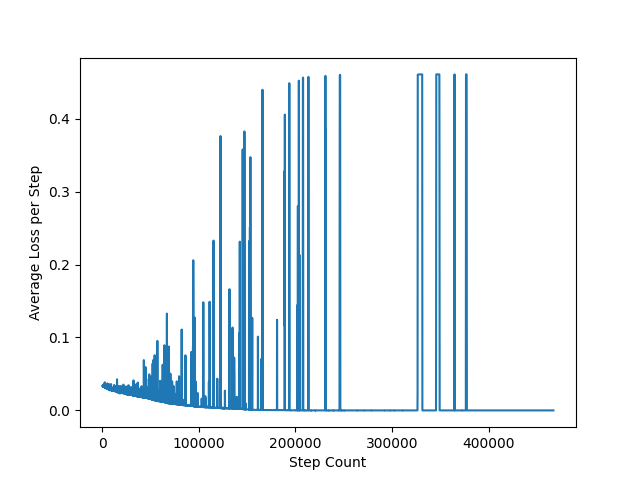
\includegraphics[width=12cm]{Images/Evaluation/NullActionFlatline.png}
            \caption*{Neural Network flatlining towards 0 loss by only picking "Noop"}
            \caption*{Large network architecture with 49 Input Nodes} 
            \caption*{Enemies Disabled}
        \end{figure}

        I am unsure as to what the spikes are, I believe it is due to instabilities in the training architecture. Following on from this failed attempt
        to train the Network, I removed Noop from the action set. This led to overall weird results, the baseline Loss trends down, but doesnt manage to
        overall minimise it. I believe this is a sign that the simulation is too complex for the Network architecture to solve. 

        \begin{figure}[H]
            \centering
            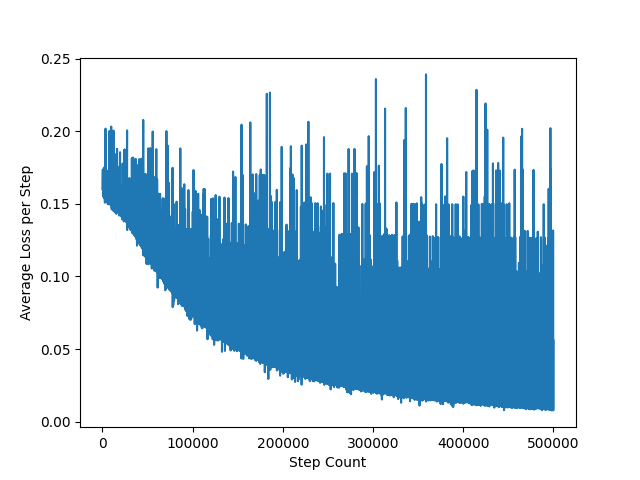
\includegraphics[width=12cm]{Images/Evaluation/AttemptedMinimiseLargeNetwork.png}
            \caption*{Neural Network attempts to minimise network but fails to solve the simulation}
            \caption*{Large network architecture with 49 Input Nodes} 
            \caption*{Enemies Disabled, Attack and Noop action disabled}
        \end{figure}

        I then enabled the enemies with the same Network architecture, this led to different results. The Network clearly places a signifcance on their
        existence, but fails to overcome them as a problem. I observed during this training session that the Agent does manage to kill enemies sometimes.
        but fails to do this consistently. I believe this might be due to the high sensory input.

        \begin{figure}[H]
            \centering
            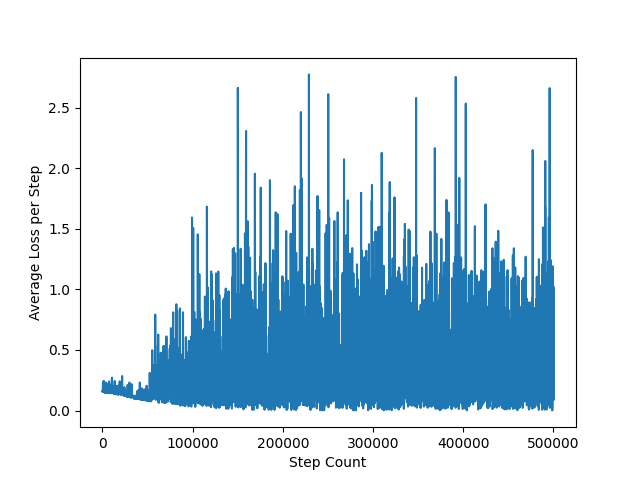
\includegraphics[width=12cm]{Images/Evaluation/EnemiesEnabled.png}
            \caption*{Neural Network struggles with Enemies}
            \caption*{Large network architecture with 49 Input Nodes} 
            \caption*{Noop action disabled}
        \end{figure}

        I also attempted training using different Network architectures, this led to much better results compared to the previous training session with 49 Inputs.
        This as stated previously may be due to the high sensory input of a larger Network. I think the 25 Input Network performs ever so slightly better than
        the 9 Input, but this may only be due to random chance.

        \begin{figure}[H]
            \centering
            \subfloat[\centering 25 Input Nodes]{{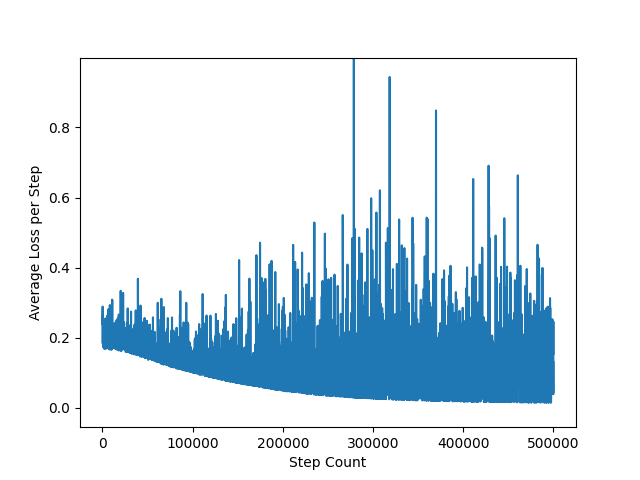
\includegraphics[width=7cm]{Images/Evaluation/25InputNetwork.png}}}
            \qquad
            \subfloat[\centering 9 Input Nodes]{{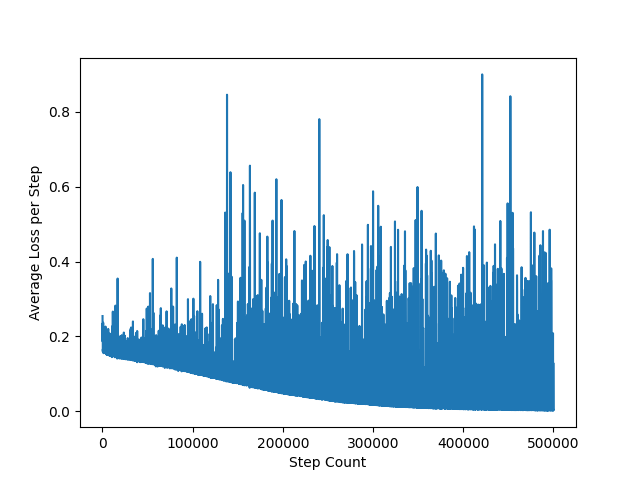
\includegraphics[width=7cm]{Images/Evaluation/9InputNetwork.png}}}
        \end{figure}

        I then chose the best performing Network out of the 3 I tested, which has 25 Inputs, and tried it with all the Activation Functions I've implemented. Previously
        I had just been using the standard Sigmoid Activation funtion. This is an attempt to find the best possible Network $\rightleftharpoons$ Activation Combination.

        \begin{figure}[H]
            \centering
            \subfloat[\centering Sigmoid Activation Function]{{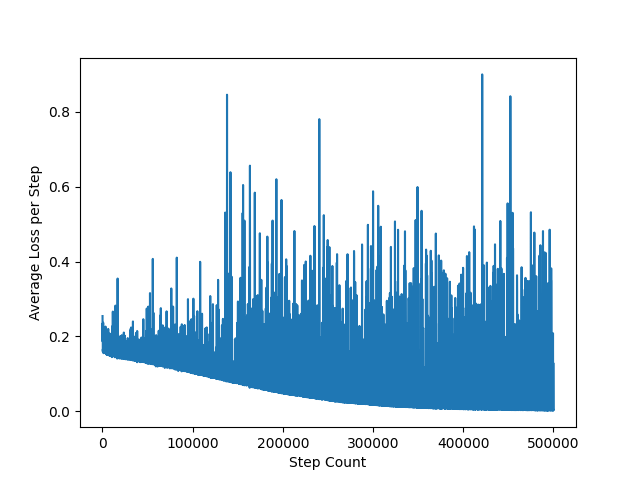
\includegraphics[width=8cm]{Images/Evaluation/9InputNetwork.png}}}
            \qquad
            \subfloat[\centering TanH Activation Function]{{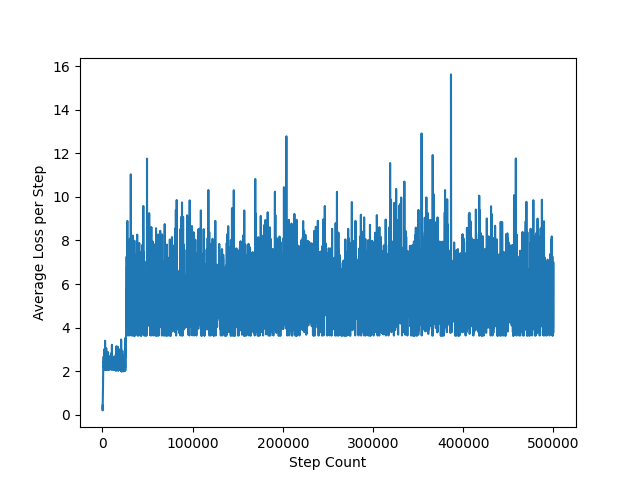
\includegraphics[width=8cm]{Images/Evaluation/9InputNetworkTanH.png}}}
            \qquad
            \subfloat[\centering ReLu Activation Function]{{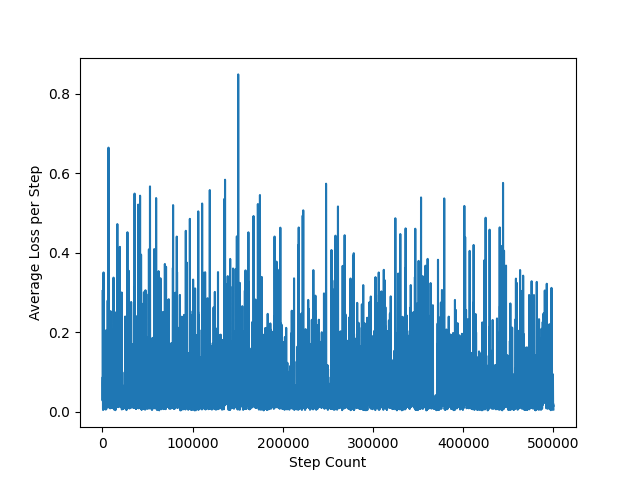
\includegraphics[width=8cm]{Images/Evaluation/9InputNetworkReLu.png}}}
            \qquad
            \subfloat[\centering Leaky ReLu Activation Function]{{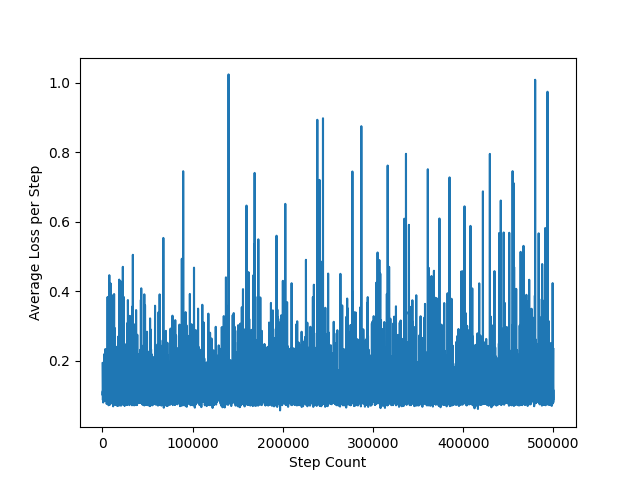
\includegraphics[width=8cm]{Images/Evaluation/9InputNetworkLeakyReLu.png}}}
        \end{figure}

        As shown above Sigmoid is clearly the best Activation Function to use for the problem. TanH exhibits weird behaviour which I can't explain. 
        ReLu and Leaky ReLu preform similarly, with Leaky ReLu being slightly better but both may as well be random. Leaving us with the best Network 
        Architecture with a layer structure of $[25,32,16,8,6]$, utilising the Sigmoid Activation Function. \\
        \vspace{0.2cm}
        In an attempt to reduce the complexity of the simulation I created, I altered the simulation slightly. I turned off the Enemies movement,
        this was an attempt to reduce the difficulty of the problem for the Agent. I also spawned 30 rather than 5 enemies at the start of a created
        world. This resulted in somewhat better results when compared to previous results, the baseline loss minimises towards 0 quicker. This is 
        definitely because the Network finds static threats easier to deal with. I also noticed in the previous test that the Agent didn't appear 
        to have a problem avoiding the Static Enemies, so I kept this for the next test.

        \begin{figure}[H]
            \centering
            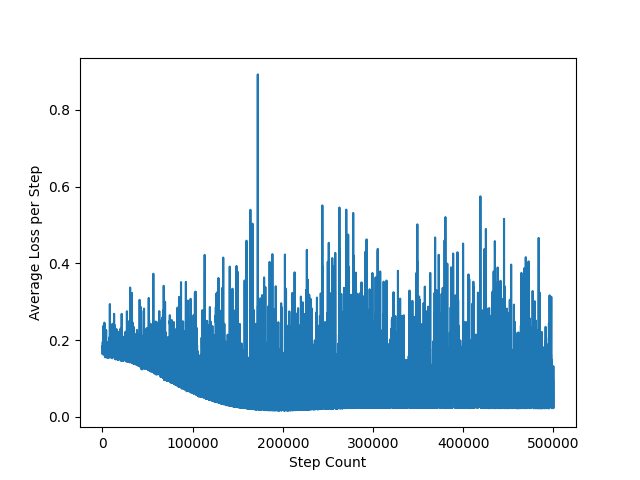
\includegraphics[width=12cm]{Images/Evaluation/StaticEnemiesExtra.png}
            \caption*{Altered Simulation Data using Static Enemies}
            \caption*{25 Input Nodes}
        \end{figure}

        This next test involved me changing the Colour of the Water to the same colour as the Enemies. I figured that this would improve the Networks
        Ability to determine what is a threat to its Survival. Instead of having to form a relationship between two colours, it was only one. This
        performed quite well in comparison to previous tests. The overall average loss is less than every other test, and shows that the Network is 
        actually capable of determining relationships between the input values and correct outputs.

        \begin{figure}[H]
            \centering
            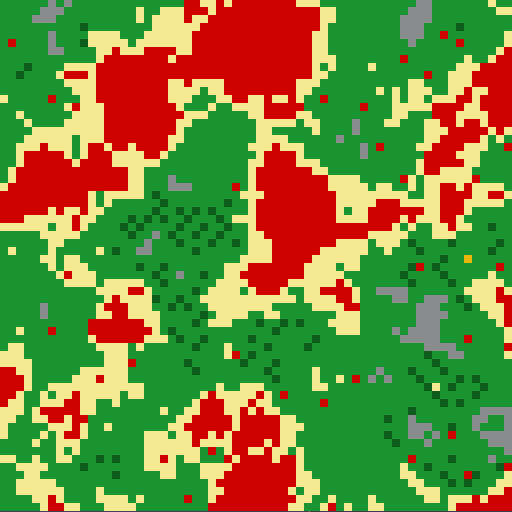
\includegraphics[width=8cm]{Images/Evaluation/RedWaterTest.PNG}
            \caption*{Altered Simulation using Static Enemies and Red Water}
            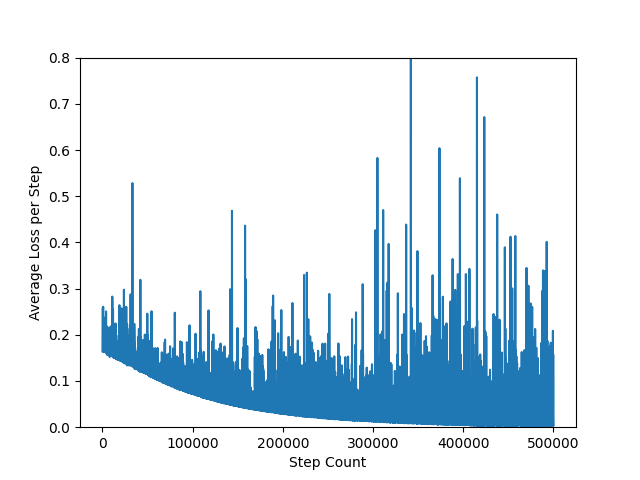
\includegraphics[width=12cm]{Images/Evaluation/RedWaterStaticExtra.png}
            \caption*{Simulation Data}
            \caption*{25 Input Nodes}
        \end{figure}

    \pagebreak
    \subsection{Answering the Proposed Questions}
        \vspace{0.2cm}
        As part of my Machine Learning Investigation I proposed the Question:

        \vspace{0.3cm}\begin{center}
        \textbf{Can I develop a Machine Learning Algorithm to survive in a pseudorandom, open-world environment?}
        \end{center}\vspace{0.3cm}

        I aimed to answer this question by designing and creating a Deep Reinforcement Learning Model utilising a Deep Neural Network, along 
        with designing a Simple Simulation for a Machine Learning Agent to survive in. \\
        \vspace{0.2cm}
        With the Machine Learning Model I implemented, the Agent was unable to fully solve the simulation. After being trained to 500000
        steps with multiple different layer structures and parameters, it fails to achieve a true solution to the problem at any given time step.
        The Average Loss of of the Network for most of my tests trends downwards, but still remains highly innacurate. The graphed data shows
        that the Average Loss (Plotted per 100 Steps) constantly peaks and drops back down to the baseline. This baseline for most of the tests
        I performed trends downwards as a curve. All the Tests Data is shown above. \\
        \vspace{0.2cm}
        Because the implemented algorithm has not managed to fully solve the problem, I have answered the sub-questions I outlined in my 
        \textit{Statement of Investigation}: \\

        \begin{itemize}
            \item The Algorithm quite clearly forms a link between specific elements in the simulation and danger, even if it doesnt manage to avoid them
            always. This can be shown by the Network managing to identify and kill the Enemies, along with performing better in my test where I altered 
            the Colour of the Water to be the same as the enemies colour. With this in place the Network manages to perform better, showing a clear
            link between the inputted colour Red and the danger associated with it. This answers the 1st sub-question, \textit{Does the Algorithm draw 
            links between specific elements and danger?}. \\
            \vspace{0.2cm}

            \item The Algorithm does manage to pickup the occasional item when attempting to solve the simulation. But it is unclear wether this is by random
            chance or if this is the intended action of the Algorithm. There is not enough evidence to suggest that the Algorithm can perform well with
            specific collection tasks of the items in the Simulation. Therefore answering the 2nd sub-question, \textit{How well does the Algorithm perform 
            with specific tasks?}. \\
            \vspace{0.2cm}

            \item I tested the Network with different Activation Functions and Layer Structures, I found that some tests performed better than others.
            This shows that the Algorithm can perform better when tuning the parameters, answering the 4th sub-question I proposed, 
            \textit{"Can I fine tune the Algorithms Parameters to get better results?"}. \\
            \vspace{0.2cm}

            \item I performed tests where I altered the simulation in order to reduce the complexity for the Algorithm. This included making the 
            Enemies Static, and changing the Colour of the Water. Both of these appeared to show the Average Loss of the Network Decrease at
            a faster rate, and a reduction of peaks in the Average Loss. The Water Colour change appeared to show the best Training results out of all
            the test results. This shows that when reducing the complexity of the problem, the Algorithm manages to better solve the given problem,
            answering the 3rd sub-question I proposed, \textit{"If the problem is altered to be simpler does the Algorithm perform better?"}.\\
            \vspace{0.2cm}
        \end{itemize}

        Overall the Algorithm implemented shows it can solve individual parts of the problem, but when combined together the complexity
        is too much for it to solve completely. I believe that the main problem here is the generalisation needed to solve a pseudorandomly
        generated environment. If the Algorithm was facing the exact same problem each time, with a linear path forward, it would most likely
        have more success when attempting to solve that problem.
    \subsection{Expert Feedback}
        \vspace{0.2cm}
        I went back to my Expert Shaun in order to collect feedback on my finalised Technical Solution. I asked him a few Questions about my
        project, paraphrased where neccesary. \\
        \vspace{0.5cm}

        \begin{enumerate}
            \item What do you think of the Program? \\
                \vspace{0.2cm}
                "Overall I think your project is incredibly visually interesting to look at, I could stare at the graphical output for hours
                just rooting for the Agent to better itself and kill the Generated Enemies. The User Inputted Parameters are easy to change
                through the json file, and it is helpful that they are locked between certain ranges to stop the User from crashing their Pc
                from allocating too much memory. The Terrain generation looks pretty good for just a 4 coloured map generated from Perlin Noise.
                The Neural Network works as intended, although it's a shame that the Machine Learning Model isn't advanced enough to 'Solve' the
                Simulation you've designed."

            \item Does my Technical Solution achieve all of the Set Goals and Objectives? \\
                \vspace{0.2cm}
                "The Program achieves all of the objectives you set out to complete, and it is clear alot of hard work went into completing your
                project. Lots of research needs to be carried out in order to understand the complexity behind Reinforcement Learning and all
                of its individual parts. Debugging this process also becomes increasingly difficult, due to the complex calculations, this 
                demonstrates you have the ability to solve problems independently. \\
                \vspace{0.2cm}
                You've also implemented an entire simulation ontop of the Dual Neural Network. Which uses more complex algorithms, this demonstrates
                you can develop multiple Vertical Slices of a project, and intertwine them together in order to create one bigger project. This
                takes planning skill and a good understanding of OOP in order to pull off." \\

            \item What Criticisms/Improvements would you suggest? \\
                \vspace{0.2cm}
                "Considering the scope of the project, youve carried out your completion of this task very well. The only suggestion I would have is
                to implement a Convolution, which might solve your Training Accuracy Problems. Otherwise a Description of your Project could be
                printed to console when the main file is run, or a 'ReadMe' text file included in the project files would useful to any users who 
                have little to no experience with Reinforcement Learning." \\

                \vspace{0.5cm}
        \end{enumerate}

        \vspace{0.5cm}
    \subsection{Evaluation of Expert Feedback}
        \vspace{0.2cm}
        I'm glad that my Expert likes my project. After putting so much work into it that is a relief. I think that his suggestions are valid, and
        in the future I might develop my project further to add a Convolution. This will hopefully boost the accuracy of my Network so I can achieve
        better training results. The ReadMe text file would also be a good addition, if I was to ever show my project publically. \\
        \vspace{0.2cm}
        Shaun has been a great use to me, such as helping me "Sanity Check" myself when my Back Propagation didn't work right off the bat (Turns out
        it was because of the complexity of the problem). This help was incredibly valuable in completing my Technically Solution. \\
        \vspace{0.5cm}
    \subsection{System Improvements}
        \vspace{0.2cm}
        Overall I am happy with my Technical Solution. I achieved all the objectives I set out to complete in my Analyis. I have definitely achieved
        my primary goal of gaining a deeper understanding about the Maths and Logic behind how Neural Networks work. This has given me a Window into
        the field of Machine Learning and Artificial Intelligence, which I intend to pursue as part of my later Studies. If I were to complete my NEA
        again I would apply Machine Learning to a different sector of problem, because Reinforcement Learning has been a tough challenge. It has been
        kindof dissapointing as well that the Network has been failed to truly solve the simulation I built. \\
        \vspace{0.2cm}
        The Improvements I would like to make to my Technical Solution are: \\
        \vspace{0.5cm}

        \begin{itemize}
            \item The Implementation of a Convolutional Neural Network was something I came across in my Initial Research and was mentioned by my Expert.
            Convolution carries out Pre-Processing on the inputted data before it is even touched by the Neural Network. This in theory would increase
            the training accuracy of my Network leading to better Results. \\
            
            \vspace{0.2cm}
            \item The Optimisation of my Matrix Class by compiling it into $C$ through the use of Cython would help speed up the training of the Neural
            Network. Due to Python being an interpretted language it is comparatively slow compared to the other programming languages I considered
            using. $C$ is a compiled language so it is comparatively alot faster, about 45 times faster according to some sources online. This could
            provide an easy way to optimise my Program without having to convert my entire Codebase into a different Language. Although I wish I
            had used a different language for my Technical Solution, I think Rust would've been the correct choice for this project. \\

            \vspace{0.2cm}
            \item An increase in complexity of my simulation would provide a greater challenge towards my Agent and Neural Network. I could add a basic
            crafting system to convert the collected Wood into a sword, or a Hunger Bar so the Agent has to collect food and water in order to survive.
            I feel as though the Network wouldnt be able to solve these problems effectively though without the implementation of my first improvement,
            a Convolutional Neural Network. \\

            \vspace{0.2cm}
        \end{itemize}
        \vspace{0.5cm}
\end{flushleft}